\documentclass[11pt,a4paper]{article}

% ---------- typography ----------
\usepackage[T1]{fontenc}
\usepackage[utf8]{inputenc}
\usepackage{newtxtext,newtxmath}
\usepackage{microtype}

% ---------- layout ----------
\usepackage{geometry}
\geometry{a4paper, top=2.6cm, bottom=2.6cm, left=2.6cm, right=2.6cm}
\usepackage{graphicx}
\usepackage{xcolor}
\usepackage{booktabs}
\usepackage{tabularx}
\usepackage{adjustbox}
\usepackage{enumitem}
\usepackage{amsmath}
\usepackage{needspace}
\usepackage{caption}
\captionsetup{font=small,labelfont=bf,skip=6pt}

\widowpenalty=10000
\clubpenalty=10000

% ---------- bibliography ----------
\usepackage[numbers,sort&compress]{natbib}
\bibliographystyle{unsrtnat}

% ---------- hyperref (last) ----------
\usepackage[
    colorlinks=true,
    linkcolor=black,
    citecolor={black!70},
    urlcolor={black!70},
    bookmarks=true,
    bookmarksnumbered=true,
    unicode=true
]{hyperref}
\usepackage{xurl}  % break URLs anywhere, after hyperref
\usepackage[htt]{hyphenat}  % allow hyphenation in \texttt

\hypersetup{
    pdftitle={Legally Subjective: Measuring the Upper Bound of Predictability in U.S. Supreme Court Decisions with Public Data and a Zero Budget},
    pdfauthor={Amine Harch el Korane},
    pdfsubject={Computational legal prediction, judicial behavior, pre-registered baselines},
    pdfkeywords={Supreme Court, judicial prediction, machine learning, pre-registration, SCDB, CourtListener}
}

\begin{document}

% ================= title block (hand-set, no \maketitle) =================
\begin{center}
{\LARGE\bfseries Legally Subjective: Measuring the Upper Bound of\\[3pt]
Predictability in U.S. Supreme Court Decisions\\[3pt]
with Public Data and a Zero Budget\par}
\vspace{14pt}
{\normalsize Amine Harch el Korane\textsuperscript{1}\par}
\vspace{2pt}
{\small\textsuperscript{1}Independent researcher.
Project and code: \href{https://github.com/Vitalcheffe/legally-subjective}{github.com/Vitalcheffe/legally-subjective}\par}
\vspace{4pt}
{\small Working paper, 29 August 2026 \textperiodcentered\ Corpus-Monde v1 (frozen 2026-08-28)\par}
\end{center}
\vspace{6pt}

% ================= abstract =================
\begin{center}
\rule{0.28\linewidth}{0.6pt}
\end{center}
\noindent\textbf{Abstract.}
Can a language model predict how a U.S. Supreme Court justice will vote
from the public case file alone, without the verdict? And if the model is
taught one justice's own writing --- a persona distilled from their past
opinions --- does it improve on that justice's \emph{future} cases? We
frame both outcomes as publishable results and report the first two
milestones of a pre-registered experiment conducted entirely on public
data at zero cost. We assemble a frozen, hash-chained corpus of 569
argued cases (OT2015--OT2023, 13 justices, 4{,}569 coded
justice$\times$case votes) by fusing CourtListener metadata with
Supreme Court Database votes. Before any model is trained, statistical
baselines fix the price of admission: predicting each justice's vote as
their modal ideological direction from the training window achieves
\textbf{63.7\%} accuracy (Wilson 95\% CI [61.3; 65.9]) at the vote
level on the held-out window --- the bar. We then train the first
structured-feature challengers (logistic regression, gradient boosting,
and interaction models over issue area, lower-court disposition, term,
and argument length, with 50 sealed 5--4 cases excluded from every
split): none beats the bar (58.6--60.4\%; McNemar $p \le 0.047$). A
feature ablation shows justice identity is the only stable signal
($-8.6$ points without it). The null result prices the residual signal:
if 63.7\% is beatable, the signal lives in the text of the cases and
opinions, which the remaining pre-registered conditions (zero-shot,
persona fine-tuning, retrieval) will test against a sealed holdout of
fifty 5--4 decisions.

\vspace{4pt}
\noindent\textbf{Keywords:} judicial prediction; Supreme Court;
pre-registration; supervised learning; attitudinal model; open data.

\begin{center}
\rule{0.28\linewidth}{0.6pt}
\end{center}
\vspace{8pt}

\section{Introduction}\label{sec:intro}

Supreme Court votes are the most consequential binary predictions in
American public life, and they are made under conditions that should
humiliate any forecaster: the inputs are thousands of pages of legal
argument, the decision rule is nine human beings, and the outcome
distribution is close enough to a coin flip that luck is difficult to
rule out. Yet a long line of work has shown that the task is not
entirely random. Statistical models built on case attributes have
predicted affirm/reverse outcomes at rates far above chance for two
decades~\citep{ruger2004,katz2017}, and the dominant theoretical
account of the Court---the attitudinal model~\citep{segal2002} ---
holds that ideology, not legal doctrine, explains most of the variance
in votes.

This paper reports the design and the first results of \emph{Legally
Subjective}, an independently conducted, zero-budget experiment that
asks a narrower and, we argue, more honest version of the prediction
question. Rather than asking how accurately a court's output can be
retrofitted by a flexible learner with centuries of data, we ask two
questions that can both fail loudly. First, is each justice's vote
predictable from the public case file alone, on a fixed, modern window,
against a pre-registered bar? Second---and this is the experiment's
live wire---if a language model is fine-tuned on one justice's own
past opinions, does it predict that justice's \emph{future} votes
better than the same model without the persona? Both answers are
publishable. If the persona helps, then judicial subjectivity leaves a
measurable textual footprint, and a justice's written voice carries
predictive information about their future decisions. If it does not,
then whatever is predictable about a justice is already captured by
their ideological direction, and the remainder is either private
deliberation or noise.

Three design commitments distinguish the project from prior work.
First, everything is pre-registered before the models see the
\emph{sealed} holdout: the baselines, the split, the metrics, and the
fifty-case test set are frozen in the repository, with the selection
seed and the SHA-256 of the sealed list published in advance. There is
no second holdout and no post hoc tuning. Second, the experiment is
built to be audited by a stranger: the corpus is assembled from public
sources with every raw file hash-chained, and every number in this
paper regenerates from scripts in the repository. Third, the budget is
zero by construction---public data, free API tiers, and free-tier
compute---which is simultaneously a constraint, a proof of
accessibility for non-institutional researchers, and a defense against
the critique that results were bought rather than earned.

The contributions of this working paper are: (i) a frozen,
provenance-complete corpus of 569 argued Supreme Court cases spanning
OT2015 through OT2023, fusing CourtListener metadata with Supreme Court
Database (SCDB) vote coding, with 98.6\% oral-argument coverage for
future multimodal conditions; (ii) pre-registered statistical
baselines, of which the strongest---per-justice modal ideological
direction---sets a vote-level bar of 63.7\% on the held-out window;
(iii) the first trained challenger, a family of structured-feature
models whose \emph{null result} is itself informative: nothing in the
pre-decision metadata adds stable signal beyond who the justice is
(Section~\ref{sec:results}); and (iv) the sealed, hash-frozen test
protocol under which the remaining conditions (zero-shot, persona
fine-tuning, retrieval) will eventually be judged
(Section~\ref{sec:protocol}).

We emphasize what this paper does not claim. It does not claim that
Supreme Court votes are unpredictable; two decades of literature and
our own baselines say otherwise. It does not report any language-model
results; the opinion-text corpus required for those conditions is
still being collected under free-tier API quotas. And it does not
treat the 63.7\% bar as trivial: as Section~\ref{sec:results} shows,
three families of supervised models failed to clear it on the same
rows, which is precisely why the bar is interesting.

\section{Related work}\label{sec:related}

\paragraph{Statistical forecasting of the Court.}
The modern line begins with the Supreme Court Forecasting Project:
\citet{ruger2004} built a conditional-choice model with input from
political science theory and, over a single term, predicted 75\% of the
Court's affirm/reverse outcomes---against 59.1\% for a panel of
legal experts. The lesson was bruising for doctrine: a small
regression with ideological covariates beat trained lawyers reading
the briefs. A decade later, \citet{katz2017} scaled the exercise with
a random forest over 628 features and nearly two centuries of
decisions (1816--2013), reporting 70.2\% accuracy at the case level
and 71.9\% at the individual vote level, and concluding that the
Court behaves in a way that is, in their words, remarkably consistent
with a machine-learning account. Both efforts, however, evaluate
\emph{in sample across history}: the models see several centuries ---
including eras with much higher unanimity rates---and predict votes
whose contemporaneous context is far removed from today's Court.

\paragraph{The attitudinal model.}
Political science supplies the theoretical prior for why such models
work. \citet{segal2002} argue that justices decide largely as
attitudes wrapped in legal reasoning: revealed ideology dominates
doctrine, and case facts matter mostly as triggers for those
attitudes. Methodologically, \citet{martin2002} estimate dynamic
ideal points for every justice since 1953, giving the field a
continuous measure of the very covariate that our strongest baseline
--- per-justice modal direction---approximates with a single bit per
justice. Our results in Section~\ref{sec:results} are, in effect, a
modern, pre-registered replication of the attitudinal prior on a
nine-term window: the ideology bit is the signal; the structured case
context is not.

\paragraph{Authorship and style.}
The persona condition is a stylometry question in modern dress.
\citet{mosteller1964} settled the authorship of the disputed
\emph{Federalist} papers with function-word frequencies; the field
they founded has since shown that individual writing style is
persistent, measurable, and hard to disguise~\citep{juola2006}. If a
justice's voice is a stable individual signature, fine-tuning a
language model on their opinions should transfer to their future
opinions; the open question---the one this experiment isolates ---
is whether that stylistic footprint carries \emph{decision-relevant}
information beyond the ideology bit, or merely rhetorical habits.

\paragraph{Language models and efficient fine-tuning.}
The tooling for the persona condition is recent. QLoRA
\citep{dettmers2023} makes full-model fine-tuning tractable on free
single-GPU tiers by quantizing the base model and training low-rank
adapters, and open-weight families such as Llama~3
\citep{llama3} provide a competent base. This is what converts the
persona question from an institutional project into a zero-budget
one: nine adapters, one per justice, trained on free-tier compute,
each sealed alongside the data that produced it.

\paragraph{Positioning.}
Against this background, the present project narrows the claim in
three ways that we believe matter for honesty of the result. The
window is short and modern (OT2015--OT2023, an era of narrow
majorities), so historical unanimity cannot inflate accuracy. The
evaluation is pre-registered and forward-holding: a sealed set of
fifty 5--4 decisions, chosen deterministically before any model
touched them, is the only arbiter of the final conditions. And the
bar is fixed \emph{before} the challengers run, at the vote level,
where the attitudinal bit is strongest---63.7\% on our window ---
so that any reported improvement is an improvement over ideology
itself, not over a straw man.

\section{Data: Corpus-Monde v1}\label{sec:data}

\subsection{Sources and fusion}

The corpus fuses two public sources, each chosen for a different
epistemic role. \emph{CourtListener} (Free Law Project)
\citep{courtlistener} supplies the case universe: dockets, dates,
parties, opinion clusters, and oral-argument audio with transcripts,
harvested from the 2026-06-30 bulk release and cross-checked against
the REST API. The \emph{Supreme Court Database} (SCDB), 2025\_01
release, justice-centered case citation file \citep{spaeth2025},
supplies the ground truth: per-justice vote directions coded by a
single, long-running editorial team whose coding conventions are
public and whose known limitations are documented in the database
itself. CourtListener defines \emph{what happened procedurally};
SCDB defines \emph{what we count as a liberal or conservative vote}.

The corpus rule is deliberately narrow: every case argued before the
Court in the window from 1 October 2015 through 30 June 2024 (terms
OT2015 through OT2023) is included if it was argued and decided with
a full opinion. Per curiams, memorandum decisions, and cases decided
without argument are excluded---not because they are uninformative,
but because the prediction task is defined over argued cases whose
written record a model could read. Applying the rule yields 569
cases. Fusion keys on docket number with sub-docket-aware matching
(a nontrivial step: consolidated dockets appear in SCDB as
comma-separated lists and occasionally in variant forms such as
original-jurisdiction numbering), and every matched pair is checked
for term and case-name agreement.

\begin{table}[t]
\centering
\caption{Corpus-Monde v1 at a glance (frozen 2026-08-28).}
\label{tab:corpus}
\small
\begin{tabular}{@{}lr@{}}
\toprule
Quantity & Value \\
\midrule
Argued cases, OT2015--OT2023 & 569 \\
Justices appearing on the bench & 13 \\
Opinions (majority, dissent, concurrence) & 1{,}778 \\
Justice$\times$case votes, coded direction & 4{,}569 \\
Cases with SCDB vote coding & 96.1\% \\
Cases with oral-argument audio + transcript & 98.6\% \\
5--4 decisions & 79 \\
\quad of which sealed for the Final Test & 50 \\
Window & 2015-10-01 to 2024-06-30 \\
\bottomrule
\end{tabular}
\end{table}

\subsection{Freeze and provenance}

The corpus is frozen: the identity of the data is fixed by a rule,
and every artifact carries the hashes of everything upstream. The
SHA-256 of every raw source file (bulk archives, API pages, the SCDB
zip) is recorded at download time; the corpus build script
recomputes them before running; and the sealed-case list (below) is
itself committed as a SHA-256 of its JSON serialization. The intent
is that a skeptical reader can verify, without trusting the author,
that the data evaluated in Section~\ref{sec:results} is the data
described here---and that nothing was edited between the freeze and
the test.

Coverage statistics are reported with their failures rather than
their successes: 22 cases carry no SCDB match at all (mostly
original-jurisdiction and consolidated matters under variant
docketing), 27 additional cases match but have no coded issue area,
and audio coverage, while high (98.6\%), is absent for a handful of
late-window matters. These gaps flow through the pipeline as explicit
missing-value categories rather than silent deletions, and the vote
analysis of Section~\ref{sec:results} simply operates on the rows
where a coded direction exists (4{,}569 of an expected
4{,}730 vote slots).

\begin{figure}[t]
\centering
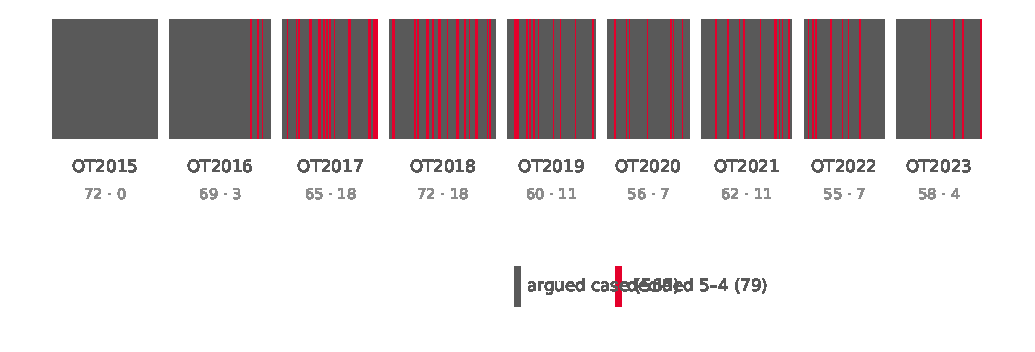
\includegraphics[width=\linewidth]{figures/fig1_corpus.pdf}
\caption{The corpus window. Each tick is one argued case, grouped by
term (counts below each group as argued~$\cdot$~5--4). Red ticks are
the 79 decisions that came down 5--4; the experiment's window is
deliberately the modern era of narrow majorities.}
\label{fig:corpus}
\end{figure}

\subsection{The bench}

Thirteen justices appear on the bench in the window, spanning three
natural cohorts: the five-justice block that opened the window
(Roberts, Scalia, Kennedy, Thomas, Ginsburg), the mid-window joiners
(Sotomayor, Kagan, Gorsuch, Kavanaugh, Barrett), and the closers
(Breyer's long service ending in 2021, Jackson arriving in 2022).
The 2020 death of Ginsburg and the two 2020 arrivals mean that no
single nine-member configuration spans the whole window; vote-level
analyses therefore condition on the justices actually sitting, and
pairwise agreement (Section~\ref{sec:results}) is computed on common
cases only, keeping the 60 pairs with at least 50 shared votes. Scalia
sits for only ten coded votes (he died in February 2016) and is
excluded from the pairwise matrix by the $n \ge 50$ rule---retained
everywhere else with his small-sample intervals displayed honestly.

\section{Protocol: pre-registration and the sealed holdout}
\label{sec:protocol}

\subsection{Split and baselines}

The experiment fixes its evaluation before fitting anything. The
corpus splits temporally: OT2015--OT2019 (2{,}314 coded votes) is the
training window, and OT2020--OT2023 is the evaluation window. All
hyper-parameter selection for the challengers of
Section~\ref{sec:results} uses grouped 5-fold cross-validation
\emph{inside the training window only}, with the group being the case
--- votes of the same case never straddle a fold boundary, because
votes within a case are correlated by construction and leaking them
across folds silently inflates validation accuracy.

On this skeleton, five statistical baselines were computed and
committed before the first challenger was trained:

\begin{itemize}[leftmargin=1.6em,itemsep=2pt]
  \item \textbf{B1---majority class}: predict the modal decision
  direction of the training window (liberal, at 51.6\% of coded
  training votes) for every vote.
  \item \textbf{B2---always conservative} (the stronger of the two
  constant policies on this window).
  \item \textbf{B3---always reverse}: predict that the Court
  upends the court below; evaluated on the subset with a clean
  affirm/reverse disposition.
  \item \textbf{B4c/B4---per-justice ideology}: predict each
  justice's vote as that justice's modal direction in the training
  window, at the case level (majority of simulated votes) and the
  vote level respectively.
  \item \textbf{B5---pairwise agreement}, a descriptive baseline
  that calibrates how differently the justices actually vote.
\end{itemize}

B4 is the bar: 63.7\% of votes on the full evaluation window (Wilson
95\% CI [61.3; 65.9]). It deserves emphasis that this bar is not a
floor to be cleared trivially---it is the accuracy of a model that
knows one bit per justice (their revealed ideological lean) and
nothing about the case. Any claim that a system ``reads the law''
must beat an adversary that cannot read at all.

\subsection{Sealing fifty of the seventy-nine}

Seventy-nine decisions in the corpus came down 5--4---the narrowest
possible majority and, folklore holds, the least predictable ones.
Fifty of them are sealed. The selection is deterministic and was
committed before any model training: the sorted list of 79 five-four
identifiers seeds a Mersenne Twister (seed derived from the SHA-256
of the sorted list), which draws 50; the resulting list is frozen by
the SHA-256 of its JSON serialization, published in the repository's
statistics file. Sealed cases are excluded from the training window,
from every cross-validation fold, and from the transparent evaluation
reported in this paper---they will be touched exactly once, by the
final conditions, in the Final Test.

The sealing rule exists to make the headline question unfakeable.
The persona condition (below) claims to extract a justice's
decision-relevant voice from their past opinions; such a claim is
only meaningful against cases the extraction pipeline never saw, and
only meaningful once. A sealed, hash-frozen, pre-registered holdout
is the cheapest device that makes retro-fitting detectable: any
post-hoc adjustment to the models after the seal is broken leaves a
git trail.

\begin{table}[t]
\centering
\caption{The four final conditions, evaluated once on the sealed
holdout.}
\label{tab:conditions}
\small
\begin{tabularx}{\linewidth}{@{}lX@{}}
\toprule
Condition & Description \\
\midrule
A---Zero-shot & An open-weight 8B language model reads the case
dossier (briefs, oral-argument transcript, question presented) and
answers with a vote direction. No learning from this corpus. \\
B---Persona & The same base model, QLoRA-fine-tuned on one
justice's \emph{past} opinions, tested on that justice's
\emph{future} and sealed cases. \\
C---Context & The same base model with retrieval of similar
earlier opinions (RAG), no fine-tuning. \\
D---Statistical & The pre-registered baselines of
Section~\ref{sec:protocol}; B4 is the bar. \\
\bottomrule
\end{tabularx}
\end{table}

\subsection{The decisive test}

The Final Test compares conditions A--D on the sealed fifty. The
pre-registered claim structure is deliberately symmetric:
\emph{if B~$>$~A} on never-seen future cases, the persona is
extractible from public text---judicial subjectivity leaves a
measurable footprint. \emph{If B~$=$~A}, the justice's personality is
not in the public data, and whatever is predictable is already
priced by ideology. Both outcomes are results; the experiment is
built so that neither can be quietly discarded.

One more protocol commitment, unusual for machine-learning papers
and central to this one: the public site that displays the
experiment's state is forbidden from showing any model output that
does not exist. Until a condition is trained, its pages show the
statistical baseline's call, labeled as such. This is not an
aesthetic preference; it is a control on the author's own incentive
to narrate success before the seal is broken.

\section{Results}\label{sec:results}

\subsection{Baselines: the price of admission}

Table~\ref{tab:baselines} and Figure~\ref{fig:baselines} report the
pre-registered baselines on the evaluation window. The ordering is
informative. The majority-class and constant policies (B1, B2) land
in the 44--56\% band---barely better than their own training-window
priors, a first sign that the evaluation window is not an easy era.
The reversal heuristic (B3) reaches 60.1\% but on the affirm/reverse
subset only, with an interval that warns against taking the point
estimate seriously. The per-justice ideology rules dominate: 55.8\%
at the case level (B4c) and \textbf{63.7\%} at the vote level (B4)
on the full evaluation window. On the transparent (sealed-excluded)
subset used for challenger comparison below, B4 scores 63.1\%
(n~$=$~1{,}522, CI [60.6; 65.5]).

\begin{table}[t]
\centering
\caption{Pre-registered baselines on the evaluation window
(OT2020--OT2023). Wilson 95\% intervals.}
\label{tab:baselines}
\small
\begin{tabular}{@{}lcc@{}}
\toprule
Baseline & Accuracy (\%) & 95\% CI \\
\midrule
B1---majority class (liberal) & 43.6 & [37.2; 50.1] \\
B2---always conservative & 56.4 & [49.9; 62.8] \\
B3---always reverse & 60.1 & [51.8; 67.9] \\
B4c---per-justice ideology, case level & 55.8 & [49.3; 62.2] \\
\textbf{B4---per-justice ideology, vote level} &
\textbf{63.7} & \textbf{[61.3; 65.9]} \\
\bottomrule
\end{tabular}
\end{table}

\begin{figure}[t]
\centering
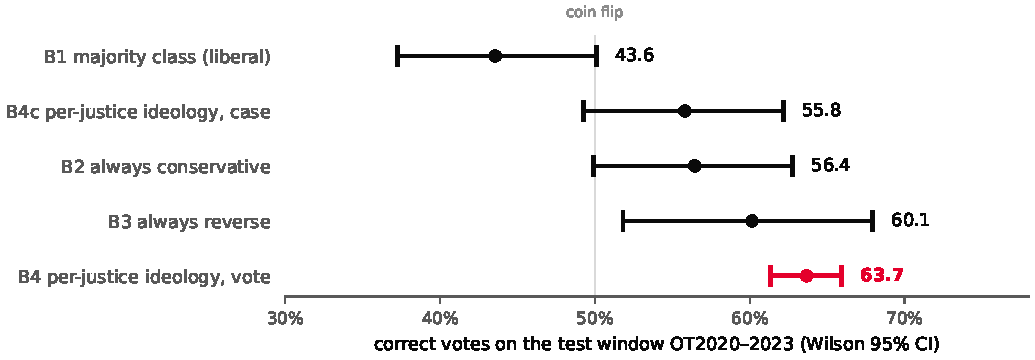
\includegraphics[width=\linewidth]{figures/fig2_baselines.pdf}
\caption{The number to beat. Wilson 95\% intervals for the five
baselines on the test window; B4 (red) is the vote-level bar of
63.7\%.}
\label{fig:baselines}
\end{figure}

\subsection{Pairwise agreement}

The descriptive baseline B5 measures how often two justices vote the
same way on their common cases. The extremes frame the scale:
Kavanaugh and Roberts agree on 94.6\% of their 333 common coded
votes (CI [91.6; 96.8]), while Sotomayor and Thomas agree on only
54.3\% of 518 (CI [50.0; 58.5])---statistically indistinguishable
from two justices flipping independent coins that share a slight
bias. Figure~\ref{fig:agreement} shows the full matrix, ordered by
mean agreement with the conservative anchor block (Thomas and
Alito). The block structure is visible without statistics: the
modern conservative five form a dark square in one corner, the
liberal three-plus in the other, and the two red-outlined extremes
are, on inspection, the two ends of the Court's ideological span.
This matrix is the empirical picture of what B4 compresses into one
bit per justice.

\begin{figure}[t]
\centering
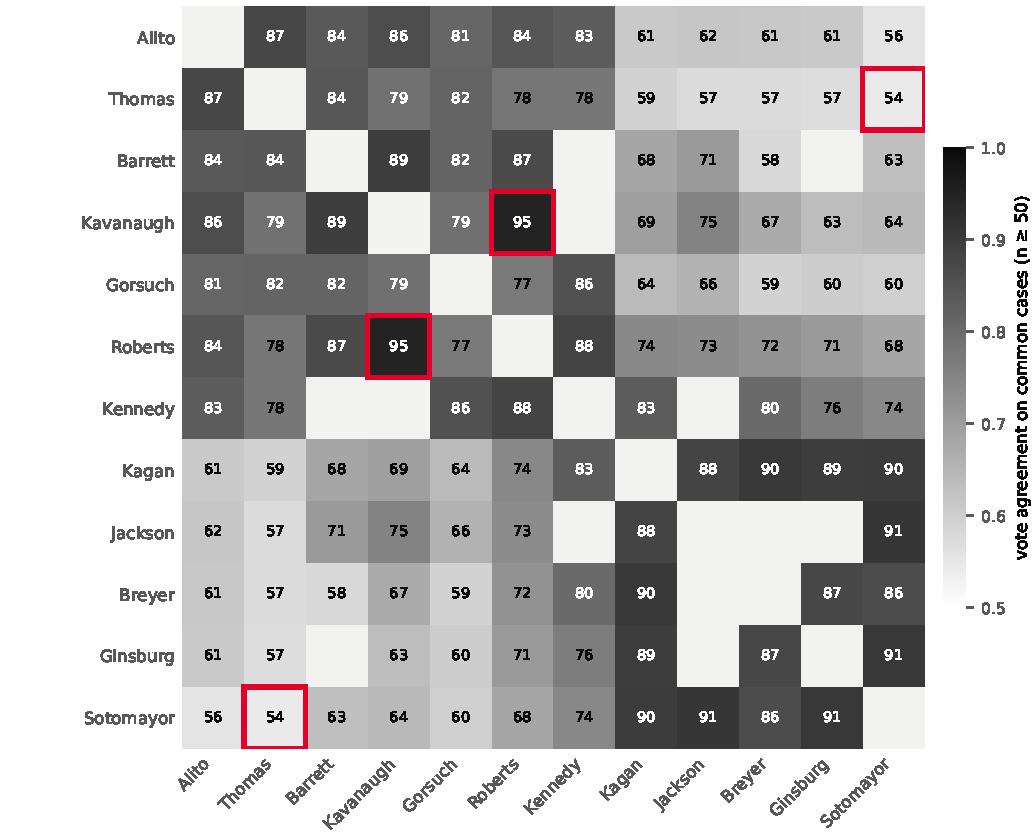
\includegraphics[width=0.92\linewidth]{figures/fig3_agreement.pdf}
\caption{Vote-level agreement across the 60 pairs with at least 50
common coded votes (values are percent agreement). Darker cells are
higher agreement; the diagonal is undefined. Red outlines mark the
closest (Kavanaugh--Roberts, 94.6\%) and widest (Sotomayor--Thomas,
54.3\%) pairs. Ordering is by mean agreement with the conservative
anchor block.}
\label{fig:agreement}
\end{figure}

\subsection{M3a: the structured challengers---and the bar holds}

The first trained condition, M3a, asks whether the structured,
pre-decision attributes of a case---issue area, lower-court
disposition, term, and oral-argument duration, joined with justice
identity---predict vote direction better than the one-bit
ideological rule. Three challengers were trained on the
sealed-excluded training window with grouped cross-validation for
all hyper-parameter choice: an additive logistic regression (M3a-LR),
the same with explicit justice$\times$issue interactions (M3a-IX),
and a histogram gradient-boosting classifier that learns
interactions natively (M3a-GB).

\begin{table}[t]
\centering
\caption{M3a challengers vs.\ the bar, transparent test
(sealed-excluded; $n=1{,}522$ rows common to all rows where B4 is
defined). McNemar exact test against B4's paired predictions.}
\label{tab:m3a}
\small
\begin{tabular}{@{}lcccc@{}}
\toprule
Model & CV (\%) & Test (\%) & 95\% CI & $p$ \\
\midrule
M3a-LR (additive) & 56.2 & 58.6 & [56.1; 61.1] & 0.002 \\
M3a-GB (boosting) & 56.1 & 59.8 & [57.3; 62.2] & 0.009 \\
M3a-IX (interactions) & 57.1 & 60.4 & [57.9; 62.8] & 0.047 \\
\textbf{B4 (bar)} &---& \textbf{63.1} & \textbf{[60.6; 65.5]} &
--- \\
\bottomrule
\end{tabular}
\end{table}

\begin{figure}[t]
\centering
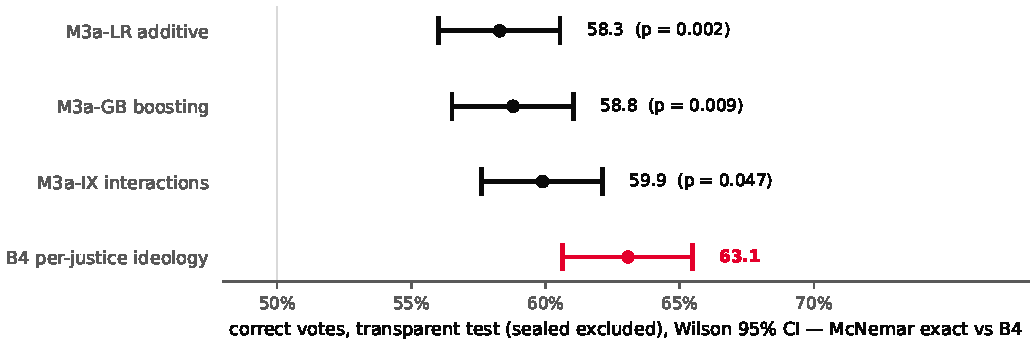
\includegraphics[width=\linewidth]{figures/fig4_m3a.pdf}
\caption{The first challenger fails against the bar. Wilson 95\%
intervals on the common rows; $p$-values are exact McNemar tests
against B4's paired predictions.}
\label{fig:m3a}
\end{figure}

Table~\ref{tab:m3a} and Figure~\ref{fig:m3a} give the result: every
challenger lands between 58.6\% and 60.4\% on the common rows, and
every comparison against B4 favors the bar (McNemar exact
$p \le 0.047$). The failure is not an artifact of regularization
strength or model family; it is robust across three families and
survives the interaction model that the site's per-justice
domain-divergence displays would suggest. It is also not a power
issue in the usual direction---the challengers are significantly
\emph{worse}, not merely insignificantly different.

The ablation in Table~\ref{tab:ablation} locates the failure
precisely. Removing justice identity from the feature set collapses
cross-validated accuracy from 56.2\% to 47.6\%---below the class
base rate---while removing any other feature group \emph{improves}
it (issue area is the most harmful to keep, at $+1.7$ points when
dropped). In other words, on this window, \emph{who} votes is
signal; \emph{what the case is about} is noise. The structured
challenger did not fail because the metadata was too thin; it
failed because the only stable generalizable structure in the data
is the attitudinal bit that B4 already uses.

\begin{table}[t]
\centering
\caption{Feature-group ablation (grouped 5-fold CV on the training
window, additive logistic regression).}
\label{tab:ablation}
\small
\begin{tabular}{@{}lc@{}}
\toprule
Feature set & CV accuracy (\%) \\
\midrule
Full (justice, issue, lc, term, duration) & 56.2 \\
drop justice identity & 47.6 \\
drop issue area & 57.9 \\
drop lower-court disposition & 56.7 \\
drop term & 56.5 \\
drop argument duration & 56.1 \\
\bottomrule
\end{tabular}
\end{table}

The case-level reading is the same. Simulating each case's outcome
as the majority of the challenger's predicted votes yields 58.3\%
(CI [51.5; 64.9]) on the transparent subset---above the case-level
ideological baseline (55.8\%), but the interval is wide enough that
the honest summary is ``not distinguishable'', and the vote-level
failure stands regardless.

\subsection{What the null prices}

Read together, the results give the experiment its current shape.
The predictable component of a justice's vote on this window is, to
the resolution that nine terms of structured data can detect, the
justice's ideological direction---exactly what the attitudinal
model predicts and exactly what B4 encodes. The additional
information that would be needed to beat 63.7\%, if it exists in
public data at all, is therefore not in the metadata: it must be in
the \emph{text}---the briefs, the transcript, the opinion language
itself. That is where the pre-registered conditions A--C operate,
and the M3a null result is what makes them the critical path rather
than a side quest: the structured ceiling is now empirically priced,
so any future claim of textual signal is a claim against a known,
pre-registered number.

\section{Discussion}\label{sec:discussion}

\subsection{Who votes beats what the case is about}

The M3a null result is a negative finding with a positive reading.
The failure of three model families to convert issue areas,
lower-court dispositions, terms, and argument lengths into votes
tells us that the mapping from case facts to outcomes is either
unstable across time or not expressible in these coarse codes. The
ablation sharpens this: keeping issue area actively hurt
generalization, which is the signature of a signal that shifted
between the training and evaluation windows---the mix and meaning
of ``economic activity'' cases in OT2015 is not the mix of OT2022.
Justice identity, by contrast, travels perfectly across the split,
because it is a property of the voter, not of the era.

This is a modern, pre-registered echo of the attitudinal model's
central claim~\citep{segal2002}, obtained with none of its
theoretical apparatus: one revealed-ideology bit per justice
carries more predictive weight than the entire structured case
file. It also explains, mechanically, why the earlier literature's
headlines sit above our bar. \citet{katz2017} report 71.9\% at the
vote level---but over 1816--2013, an era range containing long
stretches of 80--90\% unanimity that no modern model enjoys; on the
modern, 5--4-heavy window, the honest point of comparison is
closer to our setting, and the 63.7\% bar is what an
ideology-only adversary achieves when unanimity is gone.

\subsection{Why the null makes the text conditions more
interesting, not less}

Had a structured challenger cleared the bar, the persona experiment
would have been partially redundant: some of the textual signal
would already be recoverable from codes. The null result does the
opposite---it concentrates the entire residual question in the
text. If prediction above 63.7\% is possible at all on this window,
it must come from information that is written down but not coded:
the argument's framing, the questions the justices asked at oral
argument, the linguistic signature of each opinion. The persona
condition (B) tests the strongest version of that hypothesis ---
that the signature is \emph{individual} and \emph{prospective} ---
and the stylometry lineage~\citep{mosteller1964,juola2006} gives it
a principled footing: style is known to be persistent and hard to
fake, so a fine-tuned adapter is a reasonable instrument for
measuring whether style and substance are entangled.

\subsection{Calibrating expectations for the Final Test}

The sealed fifty are 5--4 decisions, which the folklore of court
watching regards as the least predictable class; and the bar was
computed on the full evaluation window, not on 5--4s specifically.
Both facts cut against the persona condition clearing B4 on the
holdout, and the honest prior is that the decisive test may return
``no difference''. We stress that this is a designed outcome, not a
failure state: a tight null on a sealed, pre-registered holdout
with per-justice adapters and audited anti-memorization checks
would be the cleanest public evidence yet that judicial
subjectivity, beyond ideology, is not extractible from the written
record---a claim that would stand regardless of how much compute
a future replicant throws at it.

\section{Limitations}\label{sec:limitations}

\paragraph{Ground truth is a single coding.}
Our outcome variable---vote direction, liberal vs.\ conservative
--- is SCDB's editorial coding, produced and maintained by a small
team applying published conventions \citep{spaeth2025}. That coding
is the field's standard, but it is one team's reading of the cases:
directional coding of some opinions (especially mixed or narrow
ones) is contestable, and the database's own documentation flags
categories with known unreliability. We did not recode anything;
all weaknesses of the coding are inherited as measurement error
that attenuates every accuracy in this paper, the bar included.

\paragraph{A short, modern window.}
Nine terms is a small epoch by the standards of the forecasting
literature, and it is deliberately the hardest modern stretch:
benches changed twice, 5--4 rates are high, and the ideological
middle (Kennedy, then Roberts) moved. Consequences are concrete ---
the training window contains no votes at all for Barrett and
Jackson, so challengers receive no signal for them, and the B4
comparison excludes them by the $n \ge 20$ rule. We consider this a
feature (the numbers describe \emph{this} Court, not a historical
average) but it bounds external validity: nothing here transfers
automatically to other eras or other courts.

\paragraph{The transparent test is exploratory.}
The M3a comparison in Section~\ref{sec:results} runs on the
non-sealed evaluation window. Although every hyper-parameter was
selected by grouped cross-validation inside the training window and
the three model families were fixed in advance, the transparent
test was run once, on data we had already seen while computing
baselines; the multiple comparisons across three challengers are
not corrected. The sealed fifty exist precisely to absorb this
residual degrees-of-freedom problem at the Final Test.

\paragraph{No text yet.}
The opinion-text corpus (M1.5) is 112 of 1{,}778 opinions deep,
dripping at free-tier API quotas of roughly five requests per
minute. Every textual condition therefore remains untested, and
this paper's null result bounds only the \emph{structured} world.
We regard the text as the live question, and we flag the risk we
cannot exclude: the eventual persona adapters may overfit
memorized opinion content rather than transferable style ---
mitigations (min-$k$\% probes, cloze audits, temporal splits
per justice) are pre-committed in the repository protocol.

\paragraph{One rater of the pipeline.}
The corpus fusion, the docket matching, and the sealed selection
were implemented and audited by a single independent researcher
with scripts, hashes, and logs---not by an institutional team.
The machinery is public and every claim regenerates from the
repository, but the human audit trail is one person deep, and we
count that as a limitation of confidence rather than of method.

\section{Ethics}\label{sec:ethics}

The experiment touches only public records: published opinions,
docket metadata, and audio of public oral arguments, all released
by the Court and mirrored by public-interest archives. No private
data, no sealed-at-source material, and no personal data beyond
the public professional conduct of public officials is used. The
justices are public figures acting in an official capacity; the
measured quantities (vote directions, agreement rates, writing
style of signed opinions) are matters of public record and public
commentary.

Two commitments go beyond data source. First, counterfactual
labels are labeled as counterfactuals: when the site or the models
display ``what the baseline would have voted'' for a case a
justice never heard (bench turnover makes this common), the row is
marked as a simulated call, never presented as a prediction the
justice could have made. Second, the project is explicitly
non-commercial: no paywall, no product, no data licensing ---
the corpus, the scripts, the trained adapters, and this paper are
published for replication and criticism. The zero-budget
constraint is partly ethical in origin: results that can only be
reproduced with institutional compute are claims that can only be
audited by institutions, and judicial-prediction claims should be
auditable by anyone.

A final note on downstream use. A high-accuracy vote predictor
would be commercially interesting to lobbyists and litigators; the
current state of the project---a 63.7\% ideological bar that
structured models fail to beat---is, we note dryly, a result
with no immediate commercial application, and we are in no hurry
to change that.

\section{Reproducibility}\label{sec:repro}

Every number in this paper regenerates from the public repository
\url{https://github.com/Vitalcheffe/legally-subjective} with three commands
and no credentials. The corpus rebuild chain is
\texttt{scripts/build\_corpus.py} (raw sources $\rightarrow$
frozen corpus with recomputed hashes); the baselines are
\texttt{scripts/m2\_baselines.py}; the M3a challengers, including
the grouped cross-validation, the McNemar tests, and the ablation,
are \texttt{scripts/m3a\_train.py}. The paper figures are produced
by \texttt{scripts/paper\_figures.py}. All randomness is seeded and
the seeds are printed in the outputs; re-running the M3a script
reproduces the numbers of Table~\ref{tab:m3a} exactly.

Provenance is structural, not narrative. The SHA-256 of every raw
source file is recorded at download; the frozen corpus recomputes
and checks them; the sealed fifty are identified by a
deterministic seeded draw whose seed derivation and resulting list
hash are both committed. A reader who wishes to verify that the
sealed list was not regenerated after training can do so from the
git history alone. The dataset rule, the known exclusions
(ghost docket groups, consolidated matters without SCDB matches),
and the coding caveats are documented in the repository's
\texttt{docs/} rather than hidden in prose.

The remaining artifact under active construction is the
opinion-text corpus (M1.5): 112 of 1{,}778 opinions collected at
the time of writing, gathered under a free API tier whose measured
quota (5 requests/minute, with multi-hour cooldown walls) makes
completion a matter of weeks rather than hours. The collection is
resumable on state, and its completion triggers the pre-committed
text conditions---at which point this paper's structured null
becomes the fixed background against which the persona question
is finally asked.

\section{Conclusion}\label{sec:conclusion}

This working paper filed the first half of a pre-registered
experiment on the predictability of Supreme Court votes. The
frozen corpus exists, is hash-chained, and is public; the
statistical baselines are committed, and the strongest of them ---
one bit of revealed ideology per justice---sets a vote-level bar
of 63.7\% on the held-out window; and the first trained challenger,
armed with everything the structured case file knows before the
decision, failed to clear the bar with three model families and a
clean ablation explaining why. The predictable part of a modern
justice's vote, to the resolution that metadata can see, is the
justice.

The second half is where the project's real question lives. The
same corpus, completed with the full text of 1{,}778 opinions,
will face the sealed fifty with a zero-shot reader, a retrieval
reader, and nine per-justice persona adapters trained on each
justice's own past words---each condition pre-registered, each
adapter audited for memorization, and each result, positive or
null, filed as a finding. The experiment was designed so that
either answer will be worth reading: a persona that beats the
zero-shot reader on unseen future cases would be the first
sealed-holdout evidence that judicial subjectivity leaves a
textual footprint; a persona that does not would be the cleanest
evidence yet that, beyond ideology, the written record keeps its
counsel. The bar is set, the seal is frozen, and the remaining
variable is the text.


\bibliography{refs}

\end{document}
